\scanpage{61}
\mspage{17}
Récapitulation des opérations élémentaires

\inserted{$(0^\circ)$ Somme \unsure{disjointe|directe}}

$1^\circ$) \uline{gommage} \inserted{\uline{total} des repères en $a$, i.e.} des repères se trouvant sur un cercle \inserted{\unsure{$C_a$}} de recollement \inserted{\unsure{les|$C_a$}}, ou \deleted{\unsure{sur un cercle}} de découpage
$\Longleftrightarrow$ suppression \unsure{d'une|de la} \deleted{partie} \inserted{$R_a$}
$(a\in A)$ $\Longleftrightarrow$ modification de $\underline r$ en le
\deleted{\unsure{de $R$ se trouvant dans une partie}}
remplaçant par $0$ en $a$.
\margin{\uline{fortement irréversible}\quad $r_a\ne0$}

$2^\circ$) \inserted{\uline{gommage partiel uniforme}: \uline{d'exposant $d_a\mid r_a$}}
Restriction des \deleted{scalaires} \inserted{groupes de $R_a$} de $\mathbb Z_a/r_a\mathbb Z$ à un
$\mathbb Z_a/r'_a\mathbb Z_a$, où $r'_a\mid r_a$ \raisebox{-.4ex}{\unsure{2|?}}
(pour $a$ fixé, il y a $r_a/r'_a=d_a$ choix possibles, où on suppose $d_a>1$ i.e. $r'_a\ne r_a$).
\margin{%
\begin{tikzpicture}[baseline=(m2label.base)]
\node[anchor=north west,inner sep=1pt,align=left] (m2label) at (0,0)
 {\uline{renforcement} de\\\uline{structure faible}\\$r_a\unsure{\ge|>}1$};
\draw ([xshift=-1pt,yshift=3pt]m2label.north west) --
 ([xshift=3pt,yshift=3pt]m2label.north east) --
 ([xshift=3pt]m2label.south east);
\node[anchor=north west,inner sep=1pt,align=left] at ([yshift=-3pt]m2label.south west)
 {\deleted{\unsure{anodin}}\\
 $r'_a\unsure{\mid|\ne}r_a$ et $r'_a\ne r_a$\\
 i.e. $d_a=\dfrac{r_a}{r'_a}\ne1$};
\end{tikzpicture}}

$3^\circ$) \deleted{Extension des}
\inserted{\uline{Surmarquage uniforme} \uline{d'exposant} $d_a>1$}
--- i.e. extension des groupes de $R_a$ de
$\mathbb Z_a/r_a\mathbb Z_a$ à $\unsure{\mathbb Z|\mathbb Z_a}/d_ar_a\mathbb Z$,
\margin{%
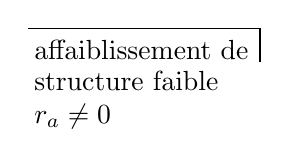
\begin{tikzpicture}[baseline=(m3label.base)]
\node[anchor=north west,inner sep=1pt,align=left] (m3label) at (0,0)
 {\uline{affaiblissement de}};
\draw ([xshift=-1pt,yshift=3pt]m3label.north west) --
 ([xshift=3pt,yshift=3pt]m3label.north east) --
 ([xshift=3pt]m3label.south east);
\node[anchor=north west,inner sep=1pt,align=left] at ([yshift=-2pt]m3label.south west)
 {structure \uline{faible}\\$r_a\ne0$};
\end{tikzpicture}}

\margin{\rule{2cm}{.3pt}\\fortement \uline{irréversible}}
\noindent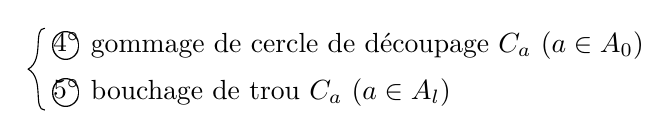
\begin{tikzpicture}[baseline=(ops.center)]
\node[anchor=west,inner sep=0pt,align=left] (ops) at (0,0)
 {\begin{tabular}{@{}l@{}}
 \textcircled{$4^\circ$} gommage de cercle de découpage $C_a$ $(a\in A_0)$\\[1.2ex]
 \textcircled{$5^\circ$} bouchage de trou $C_a$ $(a\in A_l)$
 \end{tabular}};
\draw ([xshift=-.2em]ops.north west)
 .. controls ([xshift=-.65em]ops.north west) and ([xshift=-.2em,yshift=.35em]ops.west)
 .. ([xshift=-.8em]ops.west)
 .. controls ([xshift=-.2em,yshift=-.35em]ops.west) and ([xshift=-.65em]ops.south west)
 .. ([xshift=-.2em]ops.south west);
\end{tikzpicture}

$6^\circ$) Découpage le long de $C_a$ $(a\in A_0)$ \({}^*\)
\margin{\rule{2cm}{.3pt}\\fortement irréversible si $r_a=0$, \deleted{faible} réversible = anodin si $r_a\ge1$.}

$7^\circ$) Recollement le long de $C_a,C_{a'}$
(avec $a,a'\in A_l$, $a\ne a'$, \inserted{$r_a=r_{a'}$}), via un élément de
$R_a\mathbin{\wedge}R_{a'}$.
\margin{\rule{2cm}{.3pt}\\$r_a=r_{a'}\ge1$\quad réversible = anodin}

\margin{\({}^*\) Il faudrait \inserted{peut-être} séparer $6^\circ)$ en deux, suivant que $r_a=0$ ou $r_a\ne0$ (ou \unsure{$=$|\deleted{ou}} exclure le cas $r_a=0$?)}
\mspage{60}
